% Equivalence Classes of Reals — LaTeX version
\documentclass[11pt]{article}
\usepackage[T1]{fontenc}
\usepackage[a4paper,margin=1in]{geometry}
\usepackage{hyperref}
\usepackage{enumitem}
\usepackage{amsmath,amssymb}
\usepackage{tikz}
\usetikzlibrary{arrows.meta,positioning,fit,shapes,calc}

% Macros for symbols
\newcommand{\RD}{\mathbb{R}_{\mathrm{D}}}
\newcommand{\RC}{\mathbb{R}_{\mathrm{C}}}
\newcommand{\RFC}{\mathbb{R}_{\mathrm{FC}}}
\newcommand{\RI}{\mathbb{R}_{\mathrm{I}}}
\newcommand{\RH}{\mathbb{R}_{\mathrm{H}}}
\newcommand{\Rinit}{\mathbb{R}_{\mathrm{init}}}
\newcommand{\RES}{\mathbb{R}_{\mathrm{ES}}}
\newcommand{\RCF}{\mathbb{R}_{\mathrm{CF}}}
\newcommand{\Rb}{\mathbb{R}_{b}}
\newcommand{\RSD}{\mathbb{R}_{\mathrm{SD}}}
\newcommand{\RL}{\mathbb{R}_{\mathrm{L}}}
\newcommand{\RU}{\mathbb{R}_{\mathrm{U}}}
\newcommand{\RM}{\mathbb{R}_{\mathrm{M}}}
\newcommand{\RID}{\mathbb{R}_{\mathrm{ID}}}
\newcommand{\Rterm}{\mathbb{R}_{\mathrm{term}}}
\newcommand{\RDedComp}{\mathbb{R}_{\mathrm{DedComp}}}
\newcommand{\RTarski}{\mathbb{R}_{\mathrm{Tarski}}}
\newcommand{\RCauComp}{\mathbb{R}_{\mathrm{CauComp}}}
\newcommand{\REu}{\mathbb{R}_{\mathrm{E}}}
\newcommand{\Rformal}{\mathbb{R}_{\mathrm{formal}}}

\title{Equivalence Classes of Real Numbers (Constructive, Cubical Agda)}
\author{}
\date{}

\begin{document}
\maketitle

\section*{Legend}
\begin{itemize}[leftmargin=*]
  \item Solid arrows: provable embeddings in plain Cubical Agda (no countable choice, no LEM).
  \item Dashed arrows: relationships that typically require countable choice or classical principles.
  \item ``quotient'' labels: representations coincide with Cauchy reals after quotienting the appropriate equivalence.
\end{itemize}

\section*{Diagram: Plain Cubical Agda (no CC/LEM)}

\begin{center}
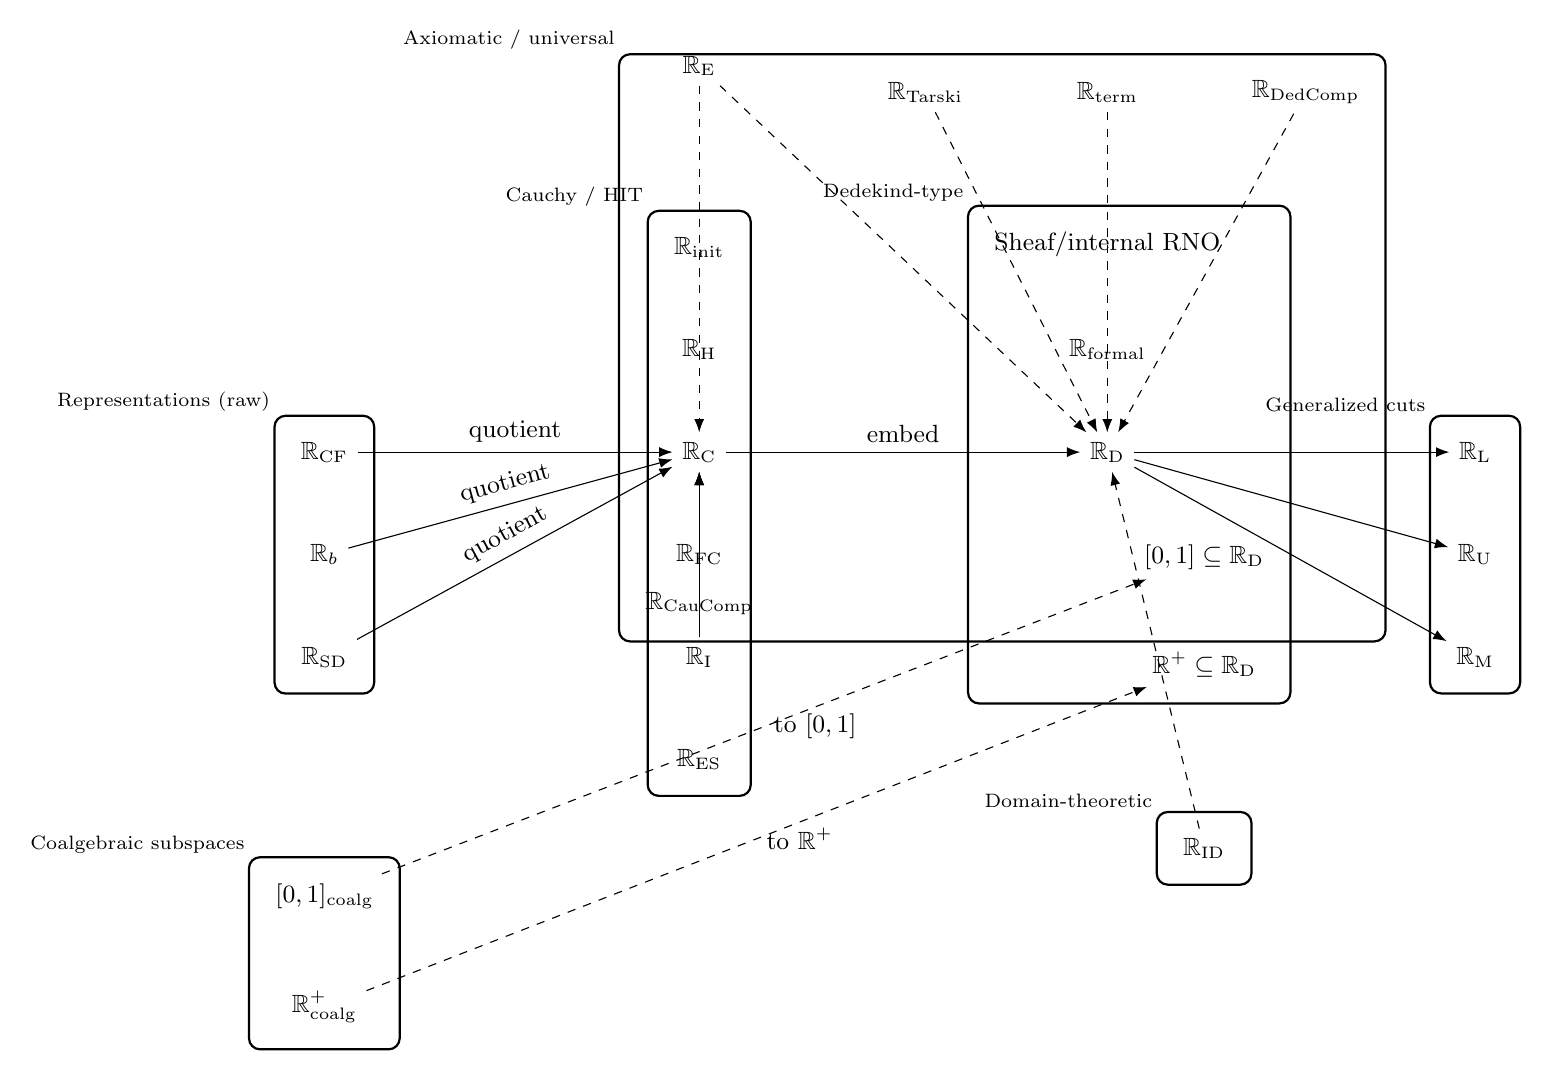
\begin{tikzpicture}[
  >=Latex,
  node distance=8mm and 12mm,
  every node/.style={font=\small},
  group/.style={draw, rounded corners, thick, inner sep=6pt},
  sublbl/.style={font=\scriptsize, inner sep=1pt},
  embed/.style={-Latex},
  cond/.style={-Latex, dashed},
]

% --- Nodes -----------------------------------------------------
% Cauchy / HIT (left-center)
\node (RC)   {\(\RC\)};
\node[below=of RC] (RFC) {\(\RFC\)};
\node[below=of RFC] (RI) {\(\RI\)};
\node[above=of RC] (RH) {\(\RH\)};
\node[above=of RH] (Rinit) {\(\Rinit\)};
\node[below=of RI] (RES) {\(\RES\)};

% Dedekind-type (center-right)
\node[right=45mm of RC] (RD) {\(\RD\)};
\node[above=of RD] (Rformal) {\(\Rformal\)};
\node[above=of Rformal] (RRNO) {Sheaf/internal RNO};
\node[below right=8mm and 0mm of RD] (Isub) {\([0,1] \subseteq \RD\)};
\node[below=of Isub] (RpSub) {\(\mathbb{R}^{+} \subseteq \RD\)};

% Representations (far left)
\node[left=40mm of RC] (RCF) {\(\RCF\)};
\node[below=of RCF] (Rb) {\(\Rb\)};
\node[below=of Rb] (RSD) {\(\RSD\)};

% Coalgebraic subspaces (bottom-left)
\node[below=25mm of RSD] (Icoalg) {\([0,1]_{\text{coalg}}\)};
\node[below=of Icoalg] (Rpcoalg) {\(\mathbb{R}^{+}_{\text{coalg}}\)};

% Generalized cuts (far right)
\node[right=40mm of RD] (RL) {\(\RL\)};
\node[below=of RL] (RU) {\(\RU\)};
\node[below=of RU] (RM) {\(\RM\)};

% Domain-theoretic (below center)
\node[below=18mm of RpSub] (RID) {\(\RID\)};

% Axiomatic / universal (top-center)
\node[above=14mm of RRNO] (Rterm) {\(\Rterm\)};
\node[right=12mm of Rterm] (RDedComp) {\(\RDedComp\)};
\node[left=12mm of Rterm] (RTarski) {\(\RTarski\)};
\node[below=14mm of RC] (RCauComp) {\(\RCauComp\)};

% Isolated / Eudoxus (top-left)
\node[above=18mm of Rinit] (REu) {\(\REu\)};

% --- Group boxes (fit) ----------------------------------------
\node[group, label={[sublbl]north west:Cauchy / HIT}] (GCB) [fit=(RC)(RFC)(RI)(RH)(Rinit)(RES)] {};
\node[group, label={[sublbl]north west:Dedekind-type}] (GDA) [fit=(RD)(Rformal)(RRNO)(Isub)(RpSub)] {};
\node[group, label={[sublbl]north west:Representations (raw)}] (GREP) [fit=(RCF)(Rb)(RSD)] {};
\node[group, label={[sublbl]north west:Coalgebraic subspaces}] (GCOA) [fit=(Icoalg)(Rpcoalg)] {};
\node[group, label={[sublbl]north west:Generalized cuts}] (GCUT) [fit=(RL)(RU)(RM)] {};
\node[group, label={[sublbl]north west:Domain-theoretic}] (GDOM) [fit=(RID)] {};
\node[group, label={[sublbl]north west:Axiomatic / universal}] (GAXI) [fit=(Rterm)(RDedComp)(RTarski)(RCauComp)] {};

% --- Proven embeddings (solid) --------------------------------
\draw[embed] (RC) -- node[above, sloped]{embed} (RD);
\draw[embed] (RFC) -- (RC);
\draw[embed] (RI) -- (RC);
\draw[embed] (RD) -- (RL);
\draw[embed] (RD) -- (RU);
\draw[embed] (RD) -- (RM);

% Representations quotient to Cauchy
\draw[embed] (RCF) -- node[above, sloped]{quotient} (RC);
\draw[embed] (Rb) -- node[above, sloped]{quotient} (RC);
\draw[embed] (RSD) -- node[above, sloped]{quotient} (RC);

% Coalgebraic to subspaces (caveats)
\draw[cond] (Icoalg) -- node[right]{to \([0,1]\)} (Isub);
\draw[cond] (Rpcoalg) -- node[right]{to \(\mathbb{R}^{+}\)} (RpSub);

% Axiomatic / domain / eudoxus — conditional or unknown
\draw[cond] (Rterm) -- (RD);
\draw[cond] (RDedComp) -- (RD);
\draw[cond] (RTarski) -- (RD);
\draw[cond] (RCauComp) -- (RC);
\draw[cond] (RID) -- (RD);
\draw[cond] (REu) -- (RC);
\draw[cond] (REu) -- (RD);

\end{tikzpicture}
\end{center}

\section*{Diagram: With Countable Choice (illustrative collapse)}

\begin{center}
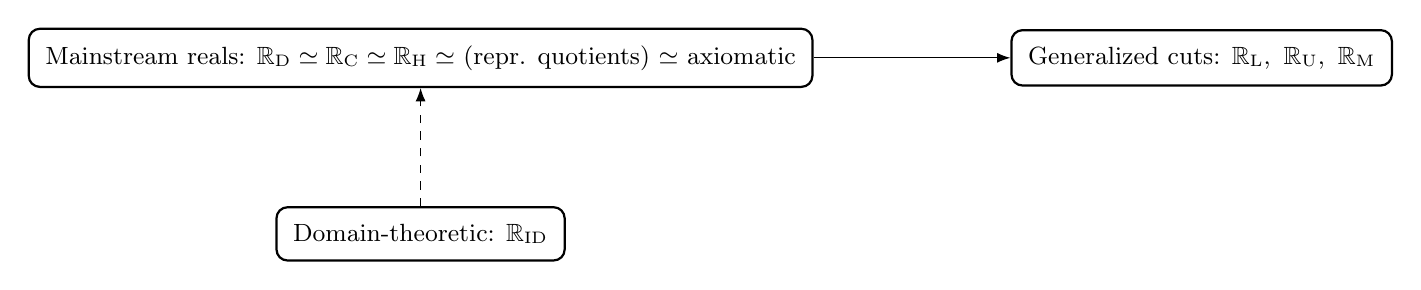
\begin{tikzpicture}[
  >=Latex,
  every node/.style={font=\small},
  group/.style={draw, rounded corners, thick, inner sep=6pt},
  cond/.style={-Latex, dashed}
]

\node[group] (Main) {Mainstream reals: $\RD \simeq \RC \simeq \RH \simeq$ (repr. quotients) $\simeq$ axiomatic};
\node[group, right=25mm of Main] (Cuts) {Generalized cuts: $\RL,\ \RU,\ \RM$};
\node[group, below=15mm of Main] (Dom) {Domain-theoretic: $\RID$};

\draw[-Latex] (Main) -- (Cuts);
\draw[cond] (Dom) -- (Main);

\end{tikzpicture}
\end{center}

\section*{Summary: Agreements}
\begin{itemize}[leftmargin=*]
  \item Canonical embedding $\RC \to \RD$ is provable; the reverse is not in Cubical Agda without countable choice.
  \item Representation streams (continued fractions, base-$b$, signed digits) require quotienting to address non-unique encodings; their quotients align with Cauchy-style reals.
  \item Lower/Upper/MacNeille reals are weaker objects (not fields) and sit below the mainstream reals.
\end{itemize}

\section*{Summary: Corrections / Cautions}
\begin{itemize}[leftmargin=*]
  \item Embeddings go $\RD \to \RL,\ \RU$ by taking lower/upper cuts; the reverse is not constructive.
  \item Place $\RES$ with Cauchy-type (the Cauchy closure inside $\RD$), not with Dedekind-type.
  \item Keep $\RH$ and $\Rinit$ together and distinct from $\RD$ (they coincide only with extra principles).
  \item Treat $\RID$ as domain-theoretic and distinct in plain Cubical Agda; do not assert equivalence to $\RD$ without additional structure.
  \item Signed-digit/base-$b$/continued-fraction representations coincide with Cauchy only after quotienting and with suitable moduli.
\end{itemize}

\section*{Recommended Partition (plain Cubical Agda)}
\begin{itemize}[leftmargin=*]
  \item Dedekind-type: $\RD$, $\Rformal$, Sheaf/internal RNO.
  \item Cauchy/HIT-type: $\RC$, $\RFC$, $\RI$, $\RH$, $\Rinit$, and (axiomatization) $\RCauComp$.
  \item Escardó--Simpson: $\RES$ (Cauchy closure inside $\RD$; group with Cauchy-type).
  \item Representations (raw, quotient to Cauchy): $\RCF$, $\Rb$, $\RSD$.
  \item Coalgebraic subspaces: $[0,1]_{\text{coalg}}$, $\mathbb{R}^{+}_{\text{coalg}}$ (subspaces of $\RD$ with constructive caveats).
  \item Generalized cuts: $\RL$, $\RU$, $\RM$ (weaker, not fields).
  \item Domain-theoretic: $\RID$ (related but not provably equivalent to $\RD$).
  \item Axiomatic/universal: $\Rterm$, $\RDedComp$, $\RTarski$ (and $\RCauComp$ if not grouped above) --- classically collapse with mainstream reals.
  \item Isolated/uncertain: $\REu$ (Eudoxus), pending additional principles for equivalence.
\end{itemize}

\section*{ASCII Fallback}
\begin{verbatim}
Representations (raw) --quotient--> RC --embed--> RD --embed--> RL, RU, RM
     |                               \
     |                                \-- (subspaces) [0,1], R+ (via coalgebras; caveats)
     +-- R_CF, R_b, R_SD

Cauchy/HIT-type: RC, RFC, RI, [RH, R_init (distinct from RD constructively)], RES

Axiomatic: R_term, R_DedComp, R_Tarski, R_CauComp  ... (classically collapse to mainstream)

Domain-theoretic: R_ID  ... (related to RD; not provably equivalent)

Eudoxus: R_E  ... (isolated; classically related to Cauchy/Dedekind)
\end{verbatim}

\end{document}

